\chapter{Entorno Empresarial}
\thispagestyle{empty} % Quitar el número

En este capítulo se describe el entorno empresarial en el cual tuvo lugar el desarrollo del proyecto de pasantía, la empresa \gls{FKC} filial de Frankfurt.

\section{Fischer, Knoblauch \& Co.}

Es un proveedor de servicios multimedia especializado en el área de aprendizaje electrónico. Está presente en Frankfurt y Munich en Alemania así como en Basel, Suiza. Fundada en 1996 por Guy Fischer y Thomas Knoblauch.

Proveen consultoría en la integración y ampliación del aprendizaje electrónico a compañías de diversos sectores en Alemania y Bélgica. Se encargan de sugerir la elección de tecnologías, concepción del plan de aprendizaje, didácticas y metodología de la enseñanza, producción del contenido audiovisual, hasta la integración de la solución en el ambiente del cliente. 

Si una compañía requiere enseñar una cierta habilidad a sus empleados contacta a un proveedor de servicios de aprendizaje electrónico, \gls{FKC} los ayuda a integrar un plan aprendizaje a su empresa, que se ven materializados en entrenamientos basados en la web. 

\gls{FKC} también posee un Sistema de Gestión de Aprendizaje, la pieza de \emph{software} en la que el pasante trabajó, que es personalizable y permite la organización de estos entrenamientos creados por la empresa.

Además, \gls{FKC} haciendo uso de su departamento gráfico y programadores, también provee servicios de posicionamiento empresarial en la web, mediante la creación de páginas, logos y demás contenido multimedia que la compañía requiera. 

Sus programadores día a día se enfrentan con diversos retos informáticos en distintos lenguajes de programación. Estos pueden ser: migraciones de sistemas de bases de datos, internacionalización de sus aplicaciones que llegan a estar hasta en diez lenguajes distintos, diseño de soluciones multiplataforma y el manejo e instalación de \emph{frameworks} que faciliten la construcción de soluciones multimedia.

\section{Estructura organizacional}

En la figura \ref{fig:estructuraFKC} se muestra la estructura organizacional de \gls{FKC} Frankfurt:

\begin{figure}[h]
\begin{center}
	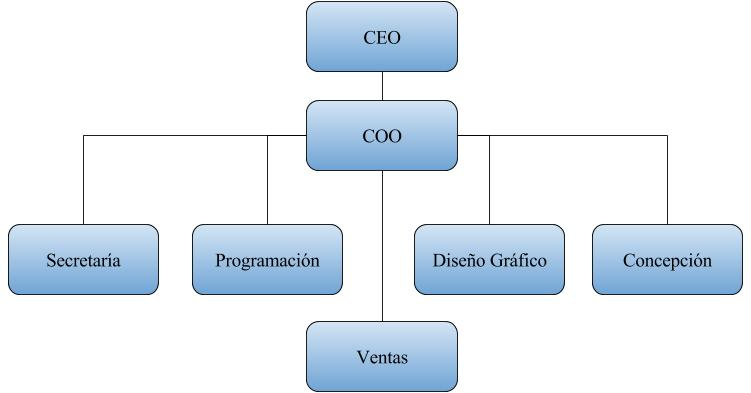
\includegraphics[width=\textwidth]{figuras/estructuraFKC.jpg}
	\caption{Estructura organizacional de \gls{FKC}.} \label{fig:estructuraFKC}
\end{center}
\end{figure}

\gls{FKC} Frankfurt es un equipo multidisciplinario donde es importante la comunicación entre los distintos \emph{stakeholders}. Los creadores de concepto se unen a los diseñadores y los programadores para plasmar fielmente los requerimientos del cliente y obtener como resultado una solución hecha a la medida.

A continuación una descripción breve de los cargos en el organigrama.

Director Ejecutivo es la persona de máxima autoridad, encargada de la gestión y dirección administrativa en la organización.

Director de Operanciones es el responsable del control de las actividades diarias de la corporación y de manejo de las operaciones. Reporta directamente al director ejecutivo.

Secretaría encargada de dar apoyo a los empleados de la empresa en cuanto a la gestión de papeleo y la comunicación de las actividades.

La cuadrilla de programación se encarga de materializar las peticiones que llegan de los demás departamentos mediante soluciones informáticas.

El grupo de diseño gráfico se encarga de generar el material multimedia junto con los integrantes del grupo de concepción y los clientes. 

El departamento de ventas se encarga del \emph{marketing} de los productos ofrecidos por \gls{FKC}.

\section{Cargo ocupado por el pasante} 

El pasante perteneció al grupo de programación que se muestra en la figura \ref{fig:estructuraFKC} donde formó parte de un equipo de 6 programadores.



